\section{HMC-LMLP}\label{sec:HMC-LMLP}

HMC-LMLP divides the learning process into a number of steps, combining MLPs individually trained for each level of the class hierarchy. The rationale is that each MLP learns something different from each other, breaking down the complex learning process into simpler~processes.

In HMC-LMLP, the MLPs are responsible for extracting local information from the instances at each level, which we believe to be useful in the classification of unlabeled instances. Our hypothesis is that different patterns can be extracted from instances in different hierarchical levels. Note that, whereas many different classifiers could be employed, we decided to choose neural networks because of the simplicity in associating a class per output neuron. Therefore, generating a multi-label prediction for a given instance is done in a straightforward fashion.

In this section, we present the proposed HMC-LMLP versions, called HMC-LMLP-Comp. These versions employ, at each level, the true labels of the instances from the previous level to augment the feature vectors. The second version is named HMC-LMLP-NoComp, since it only uses the original feature vectors to train an MLP at each level. For simplicity, all networks used in this study have a single hidden layer.

\subsection{HMC-LMLP-Comp}

Figure~\ref{fig:HMC-LMLP-Comp} illustrates the architecture of HMC-LMLP-Comp and its training process for a hierarchy with three levels. In this figure, $T_l$ are the true class labels associated to the instances at the level $l$; ${\bf X}^l$ represents the instances assigned to classes from the level $l$; $h_l$ and $O_l$ are, respectively, the hidden layer and output layer of the MLP network associated with level $l$. The matrices ${\bf W}_{1l}$ and ${\bf W}_{2l}$ represent, respectively, the weights connecting the input attributes and the neurons in the hidden layer, and the neurons in the hidden and output layers of the MLP associated with~level~$l$.

The neural network associated with the first level is trained with all training instances (${\bf X}^1$), since all instances are assigned to the classes from the first hierarchical level. At the second level, the MLP input is now the training instances that are assigned to the classes belonging to level 2 (${\bf X}^2$), combined with their true assigned classes in the first level. The advantage of using the augmented feature vector for training each MLP is the incorporation of label dependency. This process is repeated for each level of the hierarchy.

%\begin{figure*}[htbp]
%       \centering
%       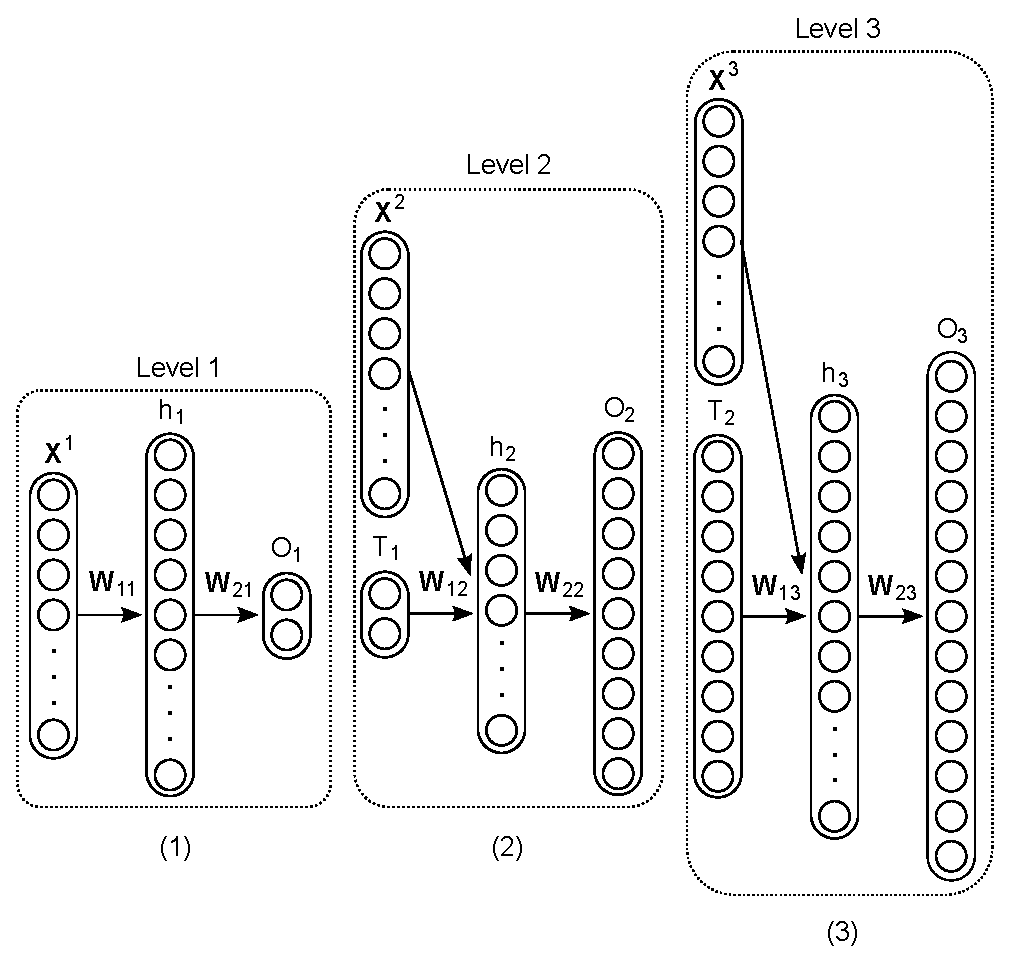
\includegraphics[scale=0.45]{HMC-LMLP-True}
%       \caption{Example of the HMC-LMLP-Comp architecture. (a) Training an MLP at the first level; (b) Using the true classes of the instances in level 1 to augment the feature vector of the instances used to train the MLP at the second level; (c) Using the true classes of the instances in level 2 to  augment the feature vector of the instances used to train the MLP at the third level.}
%       \label{fig:HMC-LMLP-True}
%\end{figure*}

As can be observed in the figure, the training process of HMC-LMLP-Comp, for each hierarchical level, can be performed in parallel, which can speed up the training process.

\subsection{HMC-LMLP-NoComp}

In HMC-LMLP-NoComp, an individual MLP is trained for each hierarchical level without employing the class labels to augment the feature vectors of the training instances. Figure~\ref{fig:HMC-LMLP-NoComp} illustrates the HMC-LMLP-NoLabels architecture and the training process. Similarly to HMC-LMLP-Comp, the training process in each level can be performed in parallel.

%\begin{figure*}[htbp]
%       \centering
%       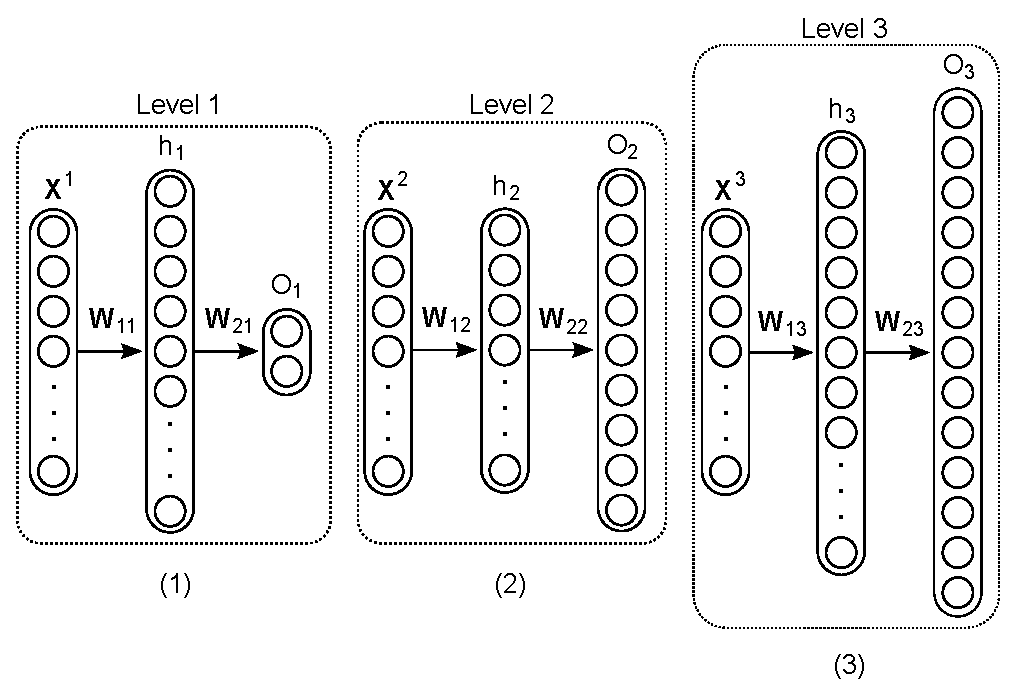
\includegraphics[scale=0.45]{HMC-LMLP-NoLabels}
%       \caption{Example of the HMC-LMLP-NoLabels architecture. (a) Training an MLP at the first level; (b) Training an MLP at the second level; (c) Training an MLP at the third level.}
%       \label{fig:HMC-LMLP-NoComp}
%\end{figure*}

\begin{figure*}[!htpb]
        \begin{subfigure}[b]{0.48\textwidth}
                \centering
                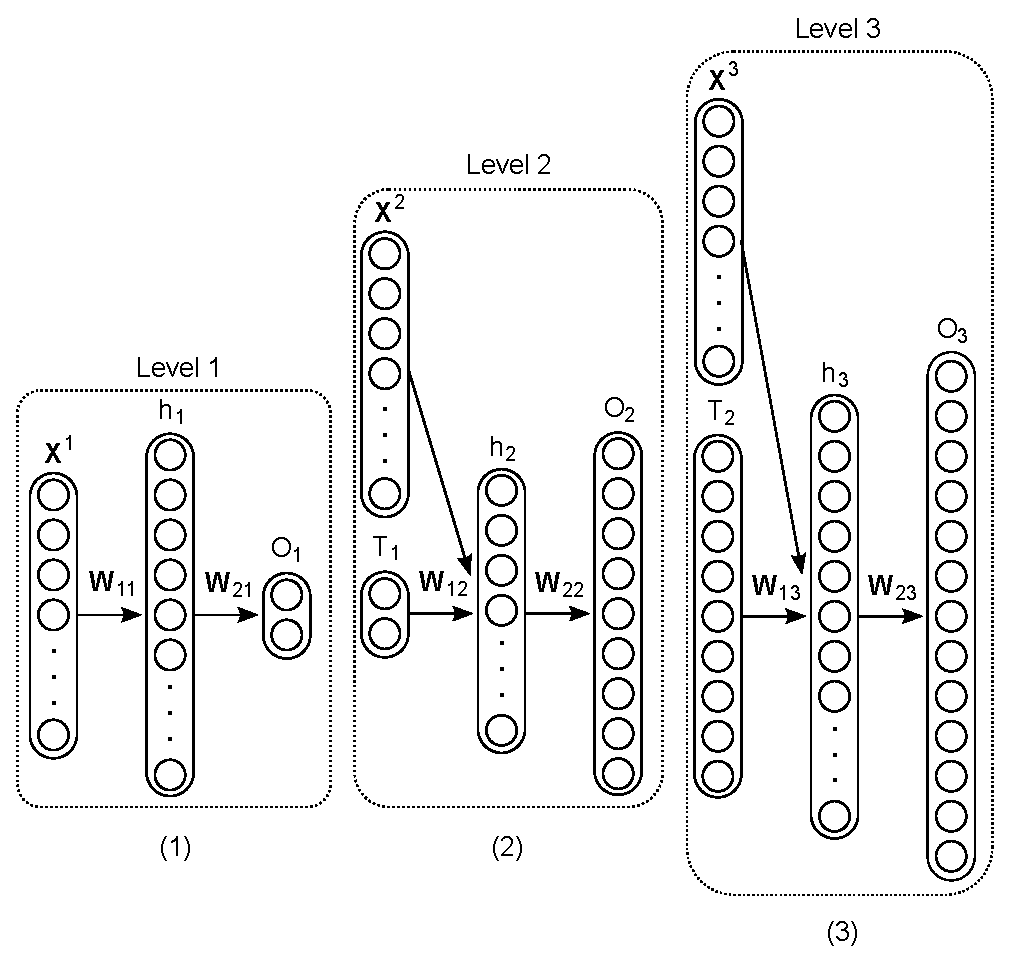
\includegraphics[scale=0.5]{HMC-LMLP-True}
                \caption{Example of the HMC-LMLP-Comp architecture. (1) Training an MLP at the first level; (2) Using the true classes of the training instances in level 1 to augment the feature vector of the instances responsible for training the MLP at the second level; (3) Using the true classes of the training instances in level 2 to augment the feature vectors which are used for training the MLP at the third level.}
                \label{fig:HMC-LMLP-Comp}
        \end{subfigure}
		\hspace{10pt}
        \begin{subfigure}[b]{0.48\textwidth}
                \centering
                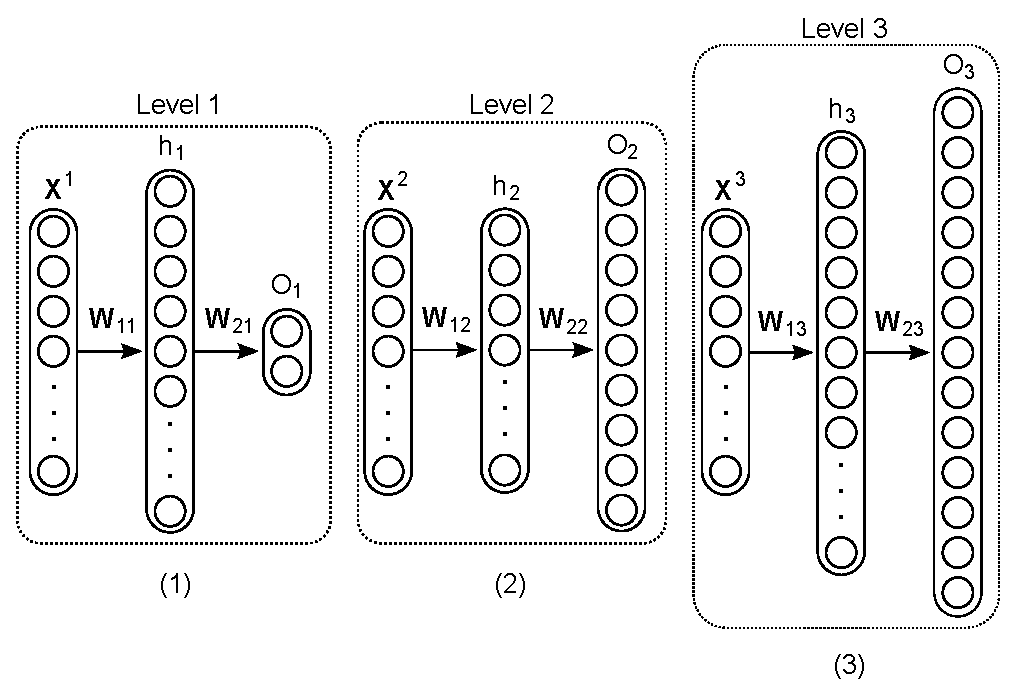
\includegraphics[scale=0.5]{HMC-LMLP-NoLabels}
                \caption{Example of the HMC-LMLP-NoComp architecture. (1) Training an MLP at the first level; (2) Training an MLP at the second level; (3) Training an MLP at the third level.}
                \label{fig:HMC-LMLP-NoComp}
        \end{subfigure}
        \caption{Example of HMC-LMLP-Comp and HMC-LMLP-NoComp architectures for a three-level hierarchy.}
        \label{fig:HMC-LMLP}
\end{figure*}

\subsection{Obtaining final predictions}

In the test phase of HMC-LMLP-Comp (i.e., when predicting a test instance), the true labels are not available. Thus, a top-down strategy is employed, in which the feature vectors that are used for training the MLP at level $l$ are augmented with the output provided by the MLP in the level $l-1$. Due to this network dependency, the testing process of HMC-LMLP-Comp cannot be performed in parallel. Instead, the predictions for each level have to be obtained sequentially. In HMC-LMLP-NoComp, the testing phase is performed by feeding all instances into all MLPs at every level. Each MLP then provides independent predictions for the instances at each level. Thus, both training and testing phases, for each level, can be performed in parallel.

%The test instance is fed to the first MLP  (first level), and predictions for this level are obtained. As the true labels are not available in the test phase, the feature vectors of the instances used to train the MLP at the second level are complemented with the output provided by the MLP associated to the first level. This augmented feature vector is then used as input to the MLP associated with the second level, whose prediction values will, once again, complement the input for the MLP at the third level. This procedure is repeated until the last MLP network, associated with the last level, is reached. Recall that the augmentation of feature vectors is not incremental, \emph{i.e.}, the feature vector of an instance being fed into an MLP associated with level $l$ is only complemented by the output from the MLP associated with level~$l-1$.

%Because we use, in each level $l$, the predictions provided in level $l-1$, the testing process of HMC-LMLP-Comp cannot be performed in parallel. Instead, the predictions for each level have to be obtained sequentially. In HMC-LMLP-NoComp, the testing phase is performed feeding all instances into all MLPs at every level. Each MLP then gives independent predictions for the instances at each level. Thus, both training and testing phases, for each level, can be performed in parallel.

After obtaining the MLP outputs values, they are tested against thresholds in order to define the predictions for each level. If the output of a given neuron $j$ is greater than or equal to a given threshold, the instance that is being classified is assigned to class $c_j$. The final classification from HMC-LMLP is given by a binary vector ${\bf{v}}$ of size $|C|$, where $C$ is the set of all classes in the hierarchy. If the output value of neuron $j$ is greater than or equal to a given threshold, the value 1 is assigned to position ${\bf v}_j$. Otherwise, the position is set to 0. Since the activation function that is used in the neurons is the logistic sigmoid function, the output values range between 0 and 1. Thus, we can make use of threshold values also ranging from 0 to 1. The larger the threshold, the lower the number of predicted classes. Conversely, the lower the threshold, the larger the number of predicted~classes.

After testing the predictions against the thresholds, there could be classification inconsistencies, \emph{i.e.}, when a subclass is predicted but its superclass is not. This problem is intrinsic to the LCL strategy \cite{Silla2010}, and for addressing this matter we employ a post-processing phase that removes all predicted classes whose superclasses were not predicted as well. 

%Fig.~\ref{fig:vectorClasses} illustrates an example of a vector of predicted classes provided by HMC-LMLP before (Fig.~\ref{fig:vectorClasses}-(a)), and after (Fig.~\ref{fig:vectorClasses}-(b)) the application of a threshold value of 0.5. Fig.~\ref{fig:vectorClasses}-(c) shows the final classification after the application of the post-processing step to correct inconsistencies (dotted circles highlight the changed bits). In the example from Fig.~\ref{fig:vectorClasses}, the final classification assigns two paths of the hierarchy to the test instance: 1.1.1.1 and~2.1.1.
%
%\begin{figure}[htbp]
%       \centering
%       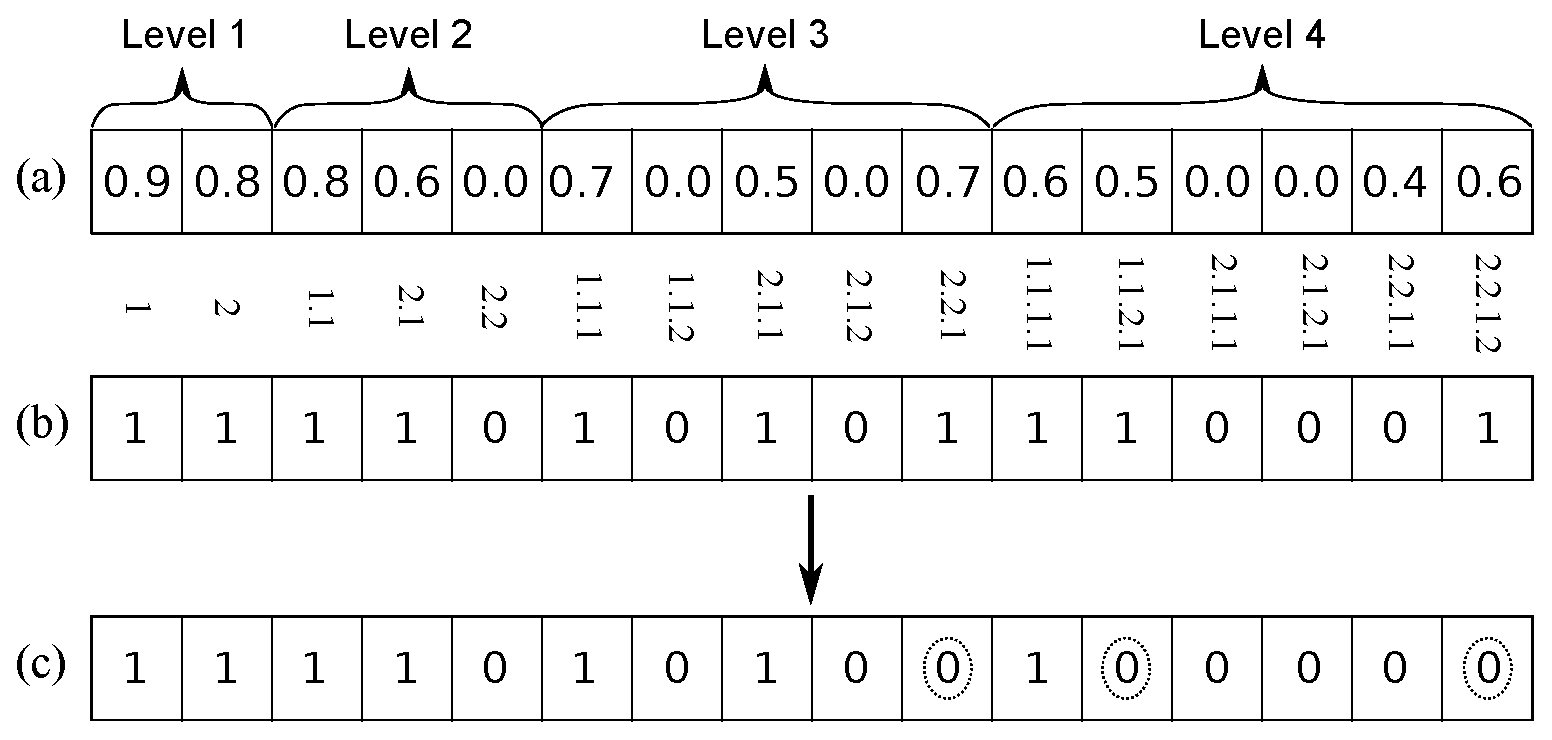
\includegraphics[scale=0.33]{VectorClasses}
%       \caption{Example of the class-predicted vector provided by HMC-LMLP. (a) Outputs from the neurons; (b) Prediction after applying a threshold value of 0.5; (c) Final classification after correcting inconsistencies.}
%       \label{fig:vectorClasses}
%\end{figure}

\subsection{Computational complexity}

Each MLP used in HMC-LMLP-Comp has a complexity of $\mathcal{O}(W_l)$, with $W_l$ being the number of weights and biases of the MLP associated with level $l$. Let $A$ be the number of attributes in the dataset, $H_l$ be the number of hidden neurons of the MLP associated with level $l$, and $O_l$ be the number of output neurons of the MLP associated with level $l$. We can thus define $W_1$ as $(A + 1) \times H_1 + (H_1 + 1) \times O_1$. From the second level onwards, $W_l$ is defined as $(O_{l-1} + A + 1) \times H_l + (H_l + 1) \times O_l$. The training cost of each MLP associated with level $l$ in HMC-LMLP-Comp is then $\mathcal{O}(W_l \times m_l \times n)$, with $m_l$ being the number of training instances assigned to classes belonging to level $l$, and $n$ the number of training epochs. In HMC-LMLP-NoComp, the computational cost is smaller, since the class labels are not used to augment the feature vectors.